
% ************* PREAMBLE

\documentclass{beamer}

% ------------- THEME

\usetheme[block=fill]{metropolis}
\usepackage{appendixnumberbeamer}
\usepackage{booktabs}
\usepackage[scale=2]{ccicons}
\usepackage{pgfplots}
\usepgfplotslibrary{dateplot}
\usepackage{xspace}
\newcommand{\themename}{\textbf{\textsc{metropolis}}\xspace}

% ------------- REFERENCES

\usepackage[backend=biber,style=apa]{biblatex}
\addbibresource{references.bib}

% ------------- OTHER PACKAGES

\usepackage[italian]{babel}
\usepackage[utf8]{inputenc}

\usepackage{stmaryrd}

\usepackage{amssymb}
\usepackage{amsmath}
\usepackage{latexsym}
\usepackage{amsthm}
\usepackage{mathabx}

\usepackage{hyperref}
\usepackage{caption}

% ------------- GENERAL INFORMATION

\title{Towards a Categorical Foundation of Deep Learning: A Survey}
\subtitle{Una rassegna di approcci categorici al \textit{deep learning}}
\author{Francesco Riccardo Crescenzi}
\institute{Alma mater studiorum - Università di Bologna \\ CdL in Matematica}


% ************* DOCUMENT

\begin{document}

\maketitle

\begin{frame}[standout]
    \Huge We are in an AI summer, but is winter coming?
\end{frame}

\begin{frame}{Problemi con il deep learning}
    \large Mancano fondamenta teoriche:
    \begin{itemize}
        \item<1-> \textbf{design ad hoc} {\footnotesize(\cite{gavranovic2024fundamental})}
        \item<2-> \textbf{complessità fine a se stessa} {\footnotesize(\cite{rahimi2017machine})}
        \item<3-> \textbf{fragilità} {\footnotesize(\cite{gavranovic2024fundamental})}
    \end{itemize}
\end{frame}

\begin{frame}{Problemi con il deep learning}
    \large La ricerca viene rallentata da:
    \begin{itemize}
        \item<1-> \textbf{research debt} {\footnotesize(\cite{olah2017research})}
        \item<2-> \textbf{mancata replicabilità} {\footnotesize(\cite{raff2019step})}
    \end{itemize}
\end{frame}

\begin{frame}[standout]
    \centering \Huge Teoria delle categorie: \\\large una lingua franca della matematica
\end{frame}

\begin{frame}{Teoria delle categorie}
    \centering La teoria delle categorie studia strutture e relazioni, e può essere vista come un'estensione del celebre \textit{Erlangen Programme}.
\end{frame}

\begin{frame}[standout]
    \centering \Huge Teoria delle categorie: \\\large una lingua franca delle scienze
\end{frame}

\begin{frame}{Teoria delle categorie applicata}
    \centering La teoria delle categorie può essere applicata con successo anche in fisica, informatica, chimica... ovunque ci sia \textbf{composizionalità} (\cite{fong2018seven}).
\end{frame}

\begin{frame}{Teoria delle categorie applicata}
    \begin{itemize}
        \item<1-> \textbf{ottiche parametriche} {\footnotesize (\cite{gavranovic2024fundamental}, \cite{cruttwell2022categorical})}
        \item<2-> \textbf{(co)algebre categoriche} {\footnotesize(\cite{gavranovicposition})}
        \item<3-> \textbf{integral transforms} {\footnotesize(\cite{dudzik2022graph}, \cite{dudzik2024asynchronous})}
        \item<4-> \textbf{functor learning} {\footnotesize(\cite{gavranovic2019compositional}, \cite{sheshmani2021categorical}, \cite{chytas2024poolingimagedatasetsmultiple})}
        \item<5-> \textbf{compositional distributional model of meaning} {\footnotesize(\cite{clark2007combining}, \cite{coecke2010mathematical}, \cite{lewis2019compositionality})}
        \item<6-> \textbf{neural circuit diagrams} {\footnotesize(\cite{abbott2023robust})}
        \item<7-> \textbf{string diagrams with universal approximators} {\footnotesize(\cite{khatri2024anatomy})}
    \end{itemize}
\end{frame}

\begin{frame}[standout]
    \huge Lenti parametriche \\\large per modellare il gradient-based learning
\end{frame}

\begin{frame}{Gradient-based learning con lenti parametriche}
    \begin{block}{DEFINIZIONE: Il costrutto $\mathbf{Para}$}
        Sia $(\mathcal{C},I,\otimes)$ una categoria monoidale strettamente simmetrica. Allora, $\mathbf{Para}_{\otimes}(\mathcal{C})$ è la $2$-categoria definita come segue.
        \begin{itemize}
          \item Le $0$-celle sono oggetti di $\mathcal{C}$.
          \item Le $1$-cells sono coppie $(P,f): A \to B$, dove $P : \mathcal{C}$ e $f: P \otimes A \to B$.
          \item The $2$-celle sono $r: (P,f) \Rightarrow (Q,g)$, dove $r: P \to Q$ è un morfismo in $\mathcal{C}$ che rispetta certe condizioni di naturalità.
        \end{itemize}
        Vedasi \cite{gavranovic2024fundamental}.
      \end{block}
\end{frame}

\begin{frame}{Gradient-based learning con lenti parametriche}
    \begin{figure}
        \begin{center}
            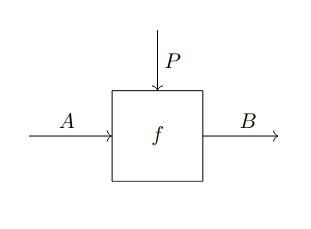
\includegraphics[width=0.5\textwidth]{figures/para.png}
            \caption*{\cite{gavranovic2024fundamental}}
        \end{center}
    \end{figure}
\end{frame}

\begin{frame}{Gradient-based learning con lenti parametriche}
    \begin{figure}
        \begin{center}
            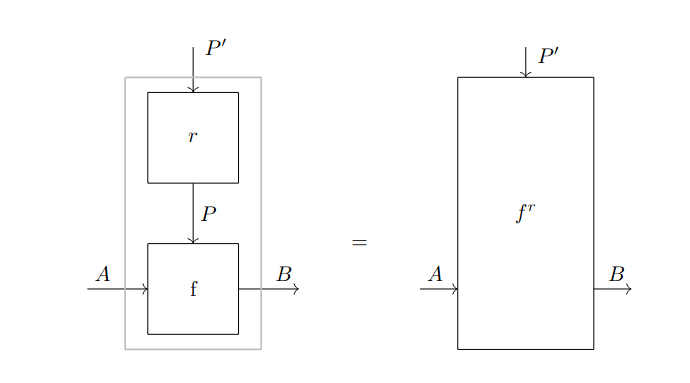
\includegraphics[width=0.7\textwidth]{figures/para_reparametrization.png}
            \caption*{\cite{gavranovic2024fundamental}}
        \end{center}
    \end{figure}
\end{frame}

\begin{frame}{Gradient-based learning con lenti parametriche}
    \begin{figure}
        \begin{center}
            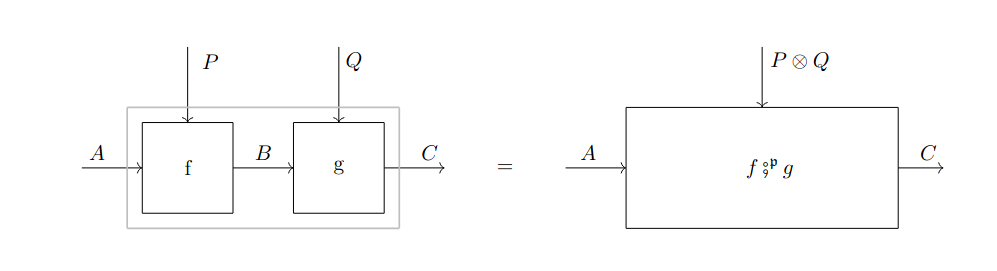
\includegraphics[width=\textwidth]{figures/para_composition.png}
            \caption*{\cite{gavranovic2024fundamental}}
        \end{center}
    \end{figure}
\end{frame}


\begin{frame}{Gradient-based learning con lenti parametriche}
    \begin{block}{DEFINIZIONE: Il costrutto $\mathbf{Lens}$}
        Sia $(\mathcal{C},1,\times)$ una categoria Cartesiana. Allora, $\mathbf{Lens}(\mathcal{C})$ è la categoria definita come segue.
        \begin{itemize}
          \item Un oggetto di $\mathbf{Lens}(\mathcal{C})$ è una coppia $\left(\begin{smallmatrix} A \\ A' \end{smallmatrix}\right)$ di oggetti di $\mathcal{C}$.
          
          \item Un morfismo $\left(\begin{smallmatrix} A \\ A' \end{smallmatrix}\right) \to \left(\begin{smallmatrix} B \\ B' \end{smallmatrix}\right)$ (anche chiamato lente) è una coppia $\left(\begin{smallmatrix} f \\ f' \end{smallmatrix}\right)$ di morfismi di $\mathcal{C}$ tali che $f: A \to B$ and $f': A \times B' \to A'$. La mappa $f$ è nota come \textit{forward pass} della lente, mentre la mappa $f'$ è nota come \textit{backward pass}.
        \end{itemize}
        Vedasi \cite{cruttwell2022categorical}.
      \end{block}
\end{frame}

\begin{frame}{Gradient-based learning con lenti parametriche}
    \begin{figure}
        \begin{center}
            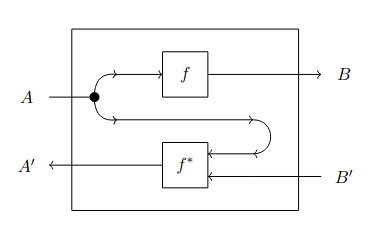
\includegraphics[width=0.7\textwidth]{figures/lens_inner_view.png}
            \caption*{\cite{cruttwell2022categorical}}
        \end{center}
    \end{figure}
\end{frame}


\begin{frame}{Gradient-based learning con lenti parametriche}
    \begin{figure}
        \begin{center}
            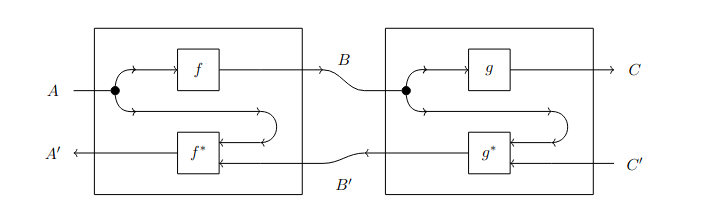
\includegraphics[width=\textwidth]{figures/lens_composition.png}
            \caption*{\cite{cruttwell2022categorical}}
        \end{center}
    \end{figure}
\end{frame}

\begin{frame}{Gradient-based learning con lenti parametriche}
    \begin{block}{DEFINIZIONE: Cartesian reverse differential category}
        Una \textit{Cartesian reverse differential category} (CRDC) $\mathcal{C}$ è una categoria Cartesiana con una struttura additiva dove è definito un operatore differenziale $\mathrm{R}$ che ha le proprietà di una \textit{reverse derivative}.
        Si vedano \cite{cockett2019reverse} e \cite{gavranovic2024fundamental}.
      \end{block}

      \begin{block}{ESEMPIO: $\mathbf{Smooth}$}
        Consideriamo $\mathbf{Smooth}$, ovvero la categoria degli spazi Euclidei e delle funzioni liscie. $\mathbf{Smooth}$ è una CRDC rispetto all'operatore
        \[\mathrm{R}[f]: (x,y) \mapsto \mathcal{J}_f(x)^Ty.\]
      \end{block}
\end{frame}


\begin{frame}{Gradient-based learning con lenti parametriche}
    \begin{block}{DEFINIZIONE: Lenti con backward pass additivo}
        Sia $\mathcal{C}$ una CRDC. Allora, definiamo la sottocategoria $\mathbf{Lens}_A(\mathcal{C})$ di $\mathbf{Lens}_A(\mathcal{C})$, i cui oggetti sono coppie $\left(\begin{smallmatrix} A \\ A' \end{smallmatrix}\right)$ e i cui morfismi hanno la forma $\left(\begin{smallmatrix} f \\ \mathrm{R}[f] \end{smallmatrix}\right)$.
        Vedasi \cite{cruttwell2022categorical}.
    \end{block}

    \begin{block}{TEOREMA: Struttura cartesiana di $\mathbf{Lens}_A(\mathcal{C})$}
        La struttura
        \[I = \left(\begin{smallmatrix} 1 \\ 1 \end{smallmatrix}\right), \quad \left(\begin{smallmatrix} A \\ A \end{smallmatrix}\right) \otimes \left(\begin{smallmatrix} B \\ B \end{smallmatrix}\right) = \left(\begin{smallmatrix} A \times B \\ A \times B \end{smallmatrix}\right)\]
        definita su $\mathbf{Lens}_A(\mathcal{C})$ è Cartesiana. Vedasi \cite{cruttwell2022categorical}.
    \end{block}
\end{frame}

\begin{frame}{Gradient-based learning con lenti parametriche}
    \begin{block}{DEFINIZIONE: Lenti parametriche}
        Sia $\mathcal{C}$ una CRDC. Allora, definiamo la categoria delle lenti parametriche su $\mathcal{C}$ come \[\mathbf{Para}_{\otimes}(\mathbf{Lens}_A(\mathcal{C})).\]
        Vedasi \cite{gavranovic2024fundamental}.
    \end{block}
\end{frame}

\begin{frame}{Gradient-based learning con lenti parametriche}
    \begin{figure}
        \begin{center}
            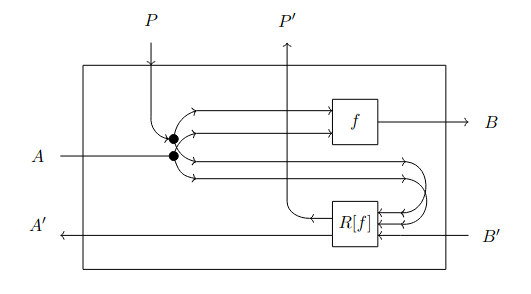
\includegraphics[width=\textwidth]{figures/parametric_lens.png}
            \caption*{\cite{cruttwell2022categorical}}
        \end{center}
    \end{figure}
\end{frame}

\begin{frame}{Gradient-based learning con lenti parametriche}
    Le lenti parametriche in $\mathbf{Para}_{\otimes}(\mathbf{Lens}_A(\mathcal{C}))$ supportano la \textit{automatic differentiation} e possono essere utilizzate per implementare il \textit{gradient-based learning} (\cite{cruttwell2022categorical}, \cite{gavranovic2024fundamental}). 
\end{frame}


\begin{frame}{Gradient-based learning con lenti parametriche}
    \begin{figure}
        \begin{center}
            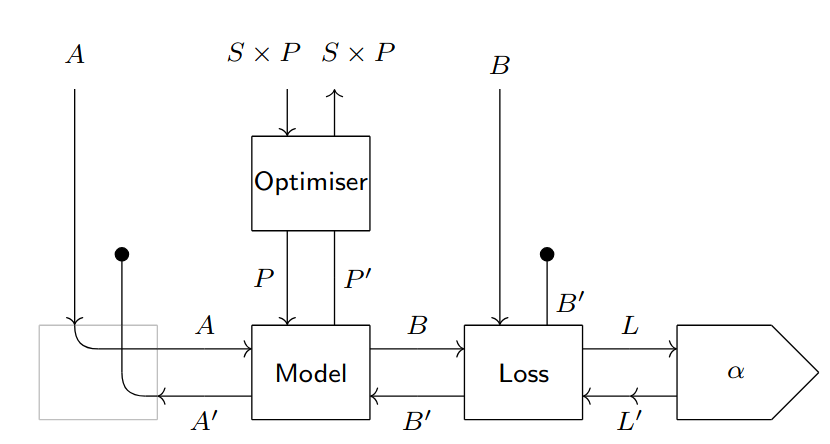
\includegraphics[width=\textwidth]{figures/lenses_supervised_learning2.png}
            \caption*{\cite{cruttwell2022categorical}}
        \end{center}
    \end{figure}
\end{frame}

\begin{frame}{Gradient-based learning con lenti parametriche}
    \begin{figure}
        \begin{center}
            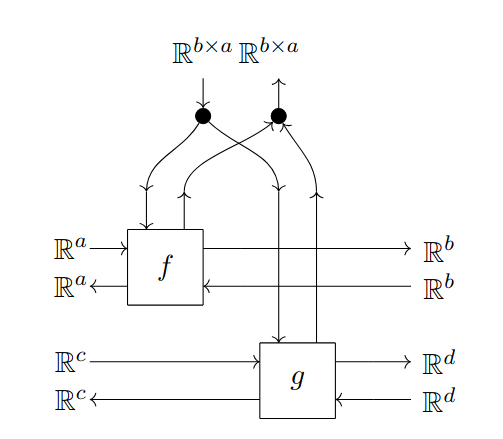
\includegraphics[width=0.5\textwidth]{figures/weight_tying.png}
            \caption*{\cite{cruttwell2022categorical}}
        \end{center}
    \end{figure}
\end{frame}

\begin{frame}{Gradient-based learning con lenti parametriche}
    \begin{figure}
        \begin{center}
            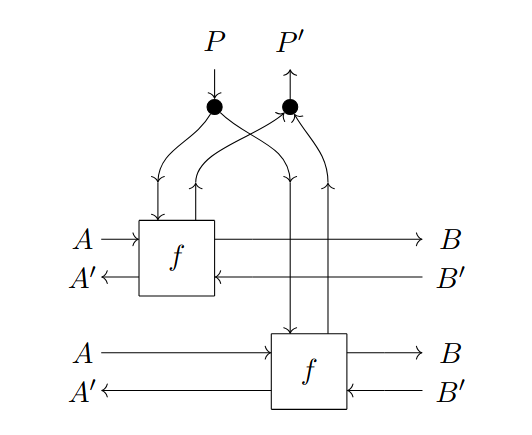
\includegraphics[width=0.5\textwidth]{figures/batching.png}
            \caption*{\cite{cruttwell2022categorical}}
        \end{center}
    \end{figure}
\end{frame}

\begin{frame}[standout]
    \huge Categorical deep learning: \\\large (co)algebre categoriche \\come teoria delle architetture
\end{frame}

\begin{frame}{Dal GDL al CDL}
    \begin{block}{\textit{Geometric deep learning}}
        Il \textit{geometric deep learning} è una teoria delle architetture di reti neurali che imita l'\textit{Erlangen Programme}, organizzando le architetture in base al concetto di equivarianza rispetto ad azioni di gruppi (\cite{bronstein2021geometric}).
    \end{block}
\end{frame}

\begin{frame}{Dal GDL al CDL}
    \begin{block}{DEFINIZIONE: Funzione equivariante}
        Sia $G$ be un gruppo e siano $(S, \cdot)$ e $(T, \ast)$ azioni di $G$. Una funzione $f: S \to T$ è equivariante rispetto a tali azioni se 
        \[f(g \cdot s) = g \ast f(s),\] 
        per ogni $s \in \mathcal{S}$ e per ogni $g \in \mathcal{G}$.
    \end{block}

    \begin{block}{ESEMPIO}
        I convolutional layers delle reti neurali rappresentano mappe invarianti rispetto a traslazioni.
    \end{block}
\end{frame}

\begin{frame}{Dal GDL al CDL}
    \begin{block}{\textit{Categorical deep learning}}
        Il \textit{categorical deep learning} è una teoria delle architetture di reti neurali che generalizza il GDL, organizzando le architetture in base al concetto di omomorfismo di (co)algebre categoriche (\cite{gavranovicposition}).
    \end{block}
\end{frame}

\begin{frame}{Dal GDL al CDL}
    \begin{block}{DEFINIZIONE: Algebra su un endofuntore}
        Sia $F: \mathcal{C} \to \mathcal{C}$ un endofuntore. Un'algebra su $F$ è una coppia $(A,a)$ dove $A$ è un oggetto di $\mathcal{C}$ e $a: F(A) \to A$ è un morfismo in $\mathcal{C}$.
    \end{block}

    \begin{block}{DEFINIZIONE: Omomorfismo di algebre}
        Siano $(A,a)$ e $(B,b)$ algebre sollo stesso endofuntore $F: \mathcal{C} \to \mathcal{C}$. Un omomorfismo di algebre $(A,a) \to (B,b)$ è un morfismo $f: A \to B$ in $\mathcal{C}$ tale che $F(f) \fatsemi b =  a \fatsemi f$.
    \end{block}
\end{frame}

\begin{frame}{Dal GDL al CDL}
    \begin{figure}
        \begin{center}
            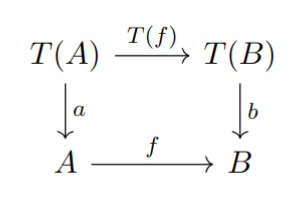
\includegraphics[width=0.5\textwidth]{figures/algebra_hom.png}
            \caption*{}
        \end{center}
    \end{figure}
\end{frame}

\begin{frame}{Dal GDL al CDL}
    Il CDL generalizza il GDL poiché le azioni di un grouppo $G$ si possono definire come algebre su una monade, e le mappe invarianti si recuperano come omomorfismi tra queste algebre.

    \vspace{5mm}

    \begin{block}{DEFINIZIONE: Monade delle azioni di $G$}
        Consideriamo l'endofuntore $G \times -: \mathbf{Set} \to \mathbf{Set}$ che mappa $A \mapsto G \times A$ e $f \mapsto G \times f$.
        La monade delle azioni di $G$ è definita dotando l'endofuntore delle transformazioni naturali di $\mu_A: (g,h,a) \mapsto (gh,a)$ e  $\eta_A: a \mapsto (e,a)$. (Vedasi \cite{gavranovicposition}.)
    \end{block}
\end{frame}

\begin{frame}{Dal GDL al CDL}
    Il CDL costruisce collega algoritmi e strutture dell'informatica classica con le reti neurali.
\end{frame}

\begin{frame}{Dal GDL al CDL}
    \begin{block}{ESEMPIO: Liste}
        Sia $A$ un insieme. Consideriamo l'endofuntore $1 + A \times -$ su $\mathbf{Set}$. Sia $\mathsf{List}(A)$ l'insieme delle liste di elementi di $A$. Allora, se $\mathsf{Nil}: 1 \to {List}(A)$ mappa l'unico oggetto di $1$ alla lista vuota e $\mathsf{Cons}: A \times \mathsf{List}(A) \to \mathsf{List}(A)$ aggiunge un elemento a una lista, $(\mathsf{List}(A), [\mathsf{Nil}, \mathsf{Cons}])$, è un algebra su $1 + A \times -$. (Esempio da \cite{gavranovicposition}.)
    \end{block}
\end{frame}

\begin{frame}{Dal GDL al CDL}
    \begin{block}{ESEMPIO: \textit{List folds}}
        Consideriamo due algebre $(\mathsf{List}(A), [\mathsf{Nil}, \mathsf{Cons}])$ e $(Z, [r_0,r_1])$ su $1 + A \times -$. Un omomorfismo $f: \mathsf{List}(A) \to Z$ tra queste due algebre deve soddisfare 
        \begin{align*}
            f(\mathsf{Nil}) &= r_0,\\
            f(\mathsf{Cons}(a,l)) &= r_1(a,f(l)). 
        \end{align*}
        Hence, $f$ è necessariamente un \textit{fold} che riduce liste di elementi di $A$ a singoli elementi di $Z$. (Esempio da \cite{gavranovicposition}.)
    \end{block}
\end{frame}

\begin{frame}{Dal GDL al CDL}
    \begin{block}{ESEMPIO: Una cella di un folding RNN}
        Consideriamo l'endofuntore $1 + A \times X:$ e la struttura cartesiana $(1, \times)$ su $\mathbf{Set}$. Su questo funtore, può essere costruito un $2$-funtore $\mathbf{Para}(1 + A \times X): \mathbf{Para}_{\bullet}(\mathbf{Set}) \to \mathbf{Para}_{\bullet}(\mathbf{Set})$. Consideriamo un algebra $(S,(P,\mathsf{Cell}))$ su tale funtore. Tramite l'isomorfismo $P \times (1 + A \times X) \cong P + P \times A \times X$, deduciamo che $\mathsf{Cell} = [\mathsf{Cell}_0, \mathsf{Cell}_1]$, dove $\mathsf{Cell}_0: P \to S$ e  $\mathsf{Cell}_1: P \times A \times S \to S$. Le funzioni $\mathsf{Cell}_0$ e $\mathsf{Cell}_1$ si possono interpretare come celle di un folding recurrent neural network. (Esempio da \cite{gavranovicposition}.)
    \end{block}
\end{frame}

\begin{frame}{Dal GDL al CDL}
    \begin{figure}
        \begin{center}
            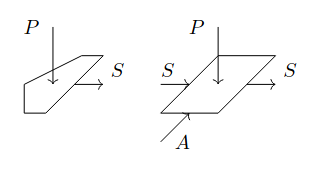
\includegraphics[width=0.7\textwidth]{figures/folding_rnn_cell.png}
            \caption*{\cite{gavranovicposition}}
        \end{center}
    \end{figure}
\end{frame}

\begin{frame}{Dal GDL al CDL}
    \begin{block}{ESEMPIO: Unrolling di un folding RNN}
        Consideriamo le due algebre $(\mathsf{List}(A), [\mathsf{Nil}, \mathsf{Cons}])$ e $(S,(P,\mathsf{Cell}))$ sull'endofuntore $\mathbf{Para}(1 + A \times X)$.
        Ora consideriamo un omomorfismo di algebre $(P,f,\Delta_P): (\mathsf{List}(A), [\mathsf{Nil}, \mathsf{Cons}]) \to (S,(P,\mathsf{Cell}))$. Si può dimostrare che una funzione $f$ così definita è l'unrolling di un folding recurrent neural network. L'algebra $(\mathsf{List}(A), [\mathsf{Nil}, \mathsf{Cons}])$ fornisce gli input della rete neurale, mentre l'algebra $(S,(P,\mathsf{Cell}))$ fornisce le celle. (Esempio da \cite{gavranovicposition}.)
    \end{block}
\end{frame}

\begin{frame}{Dal GDL al CDL}
    \begin{figure}
        \begin{center}
            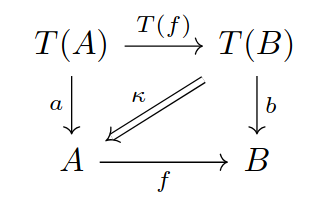
\includegraphics[width=0.5\textwidth]{figures/lax_algebra_hom.png}
            \caption*{\cite{gavranovicposition}}
        \end{center}
    \end{figure}
\end{frame}

\begin{frame}{Dal GDL al CDL}
    \begin{figure}
        \begin{center}
            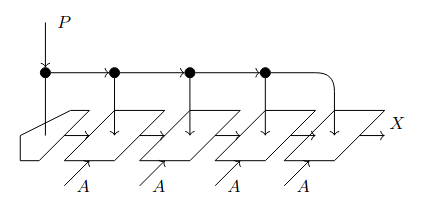
\includegraphics[width=0.8\textwidth]{figures/folding_rnn.png}
            \caption*{\cite{gavranovicposition}}
        \end{center}
    \end{figure}
\end{frame}

\begin{frame}{Dal GDL al CDL}
    \begin{figure}
        \begin{center}
            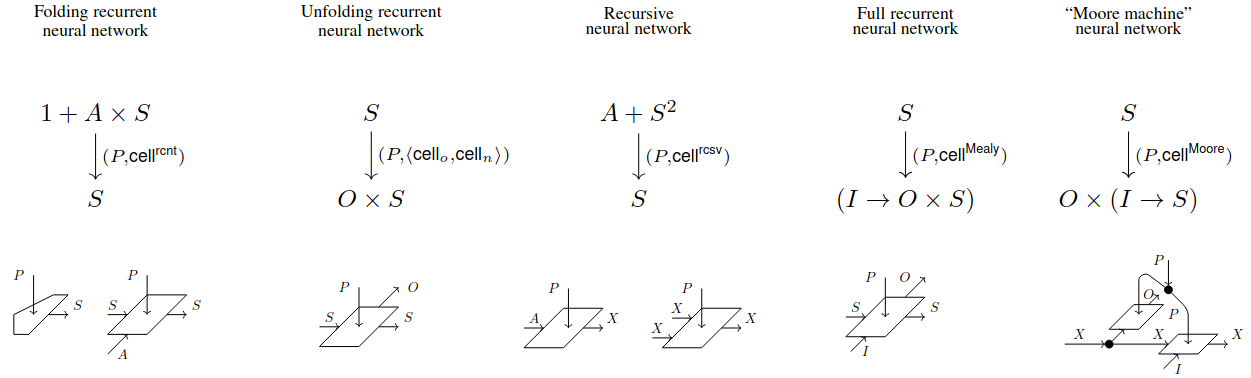
\includegraphics[width=1\textwidth]{figures/cells.png}
            \caption*{\cite{gavranovicposition}}
        \end{center}
    \end{figure}
\end{frame}

\begin{frame}[standout]
    \huge Functor learning: \\\large modelli come funtori che sfruttano la struttura dei dati
\end{frame}

\begin{frame}{Categorical representation learning}
    \begin{block}{Categorical representation learning}
        Il \textit{categorical representation learning} consiste nell'immergere funtorialmente una categoria $\mathcal{C}$ di dati in una categoria $\mathcal{R}$ di vettori latenti (\cite{sheshmani2021categorical}). 
    \end{block}

    Grazie alla funtorialità dell'embedding, il \textit{categorical representation learning} consente di preservare la struttura dei dati nello spazio latente.
\end{frame}

\begin{frame}{Categorical representation learning}
    \begin{block}{DEFINIZIONE: Struttura categorica dello spazio latente}
        tegoria i cui oggetti sono i vettori di $\mathbb{R}^n$ and tale che, per ogni $u,v$ in $\mathcal{R}$, 
        i morfismi $u \to v$ sono le matrici $M \in \mathbb{R}^{n \times n}$ tali che $v = Mu$. La composizione è l'ordinario prodotto riga per colonna e l'identità relativa a un generico $v \neq 0$ è $\mathrm{id}_v = \frac{vv^T}{|v|^2}$. L'identià relativa al vettore nullo è la matrice nulla. (Vedasi \cite{sheshmani2021categorical}.)
    \end{block}
\end{frame}

\begin{frame}{Categorical representation learning}
    Data una categoria $\mathcal{C}$ di dati, il funtore di \textit{embedding} $\mathcal{C} \to \mathcal{R}$ è realizzato da due \textbf{neural embedding layers}: il primo produce rappresentazioni degli elementi di $\mathcal{C}$ come vettori, mentre il secondo produce rappresentazioni dei morfismi di $\mathcal{C}$ come matrici. (Vedasi \cite{sheshmani2021categorical}.)
\end{frame}

\begin{frame}{Categorical representation learning}

    \begin{block}{DEFINIZIONE: Negative sampling loss}
        La \textit{objective function} utilizzata per addestrare i due \textit{layers} è la \textit{negative sampling loss}
        \[\mathcal{L} = -\mathbb{E}_{(a,b) \sim p(a,b)}\left(\log P(a \to b) + \mathbb{E}_{b' \sim p(b')}\log (1-P(a \to b'))\right),\]
        dove la probabilità che sussista una relazione $a \to b$ è misurata come
        \[P(a \to b) = \mathsf{sigmoid}\left(F\left(\bigoplus_f v_a^TM_fv_b \right)\right).\]
        (Vedasi \cite{sheshmani2021categorical}.)
    \end{block}
    
\end{frame}

\begin{frame}{Categorical representation learning}
    \begin{block}{ESEMPIO: Traduzione non supervisionata}
        Se $\mathcal{C}$ e $\mathcal{D}$ sono database di formule chimiche in inglese e cinese, rispettivamente, possiamo usare il CRL per immergere le due categorie in $\mathcal{R}$ funtorialmente. Poi si può imparare un funtore $\mathcal{F}: \mathcal{R} \to \mathcal{R}$ che preservi la struttura categorica. Tale funtore opererà la traduzione. (Esempio da \cite{sheshmani2021categorical}.)
    \end{block}
\end{frame}

\begin{frame}{Categorical representation learning}
    \begin{block}{ESEMPIO: Traduzione non supervisionata}
        Se $\mathcal{C}$ e $\mathcal{D}$ sono database di formule chimiche in inglese e cinese, rispettivamente, possiamo usare il categorical representation learning per immergere le due categorie in $\mathcal{R}$ funtorialmente. Poi si può imparare un funtore $\mathcal{F}: \mathcal{R} \to \mathcal{R}$ che preservi la struttura categorica. Tale funtore effettuerà la traduzione. $\mathcal{F}$ può essere implementato come una matrice $V_{\mathcal{F}}$ che mappa
        \begin{align*}
            v &\mapsto V_{\mathcal{F}}v,\\
            M_f &\mapsto V_{\mathcal{F}}M_f.
        \end{align*}
        (Esempio da \cite{sheshmani2021categorical}.)
    \end{block}
\end{frame}

\begin{frame}{Categorical representation learning}
    \begin{block}{ESEMPIO: Traduzione non supervisionata}
        La matrice può essere imparata minimizzando la \textit{loss function}
        \[\mathcal{L}_{\mathrm{struc}} = \sum_{f}\|V_{\mathcal{F}}M_f - M_{\mathcal{F}(f)}V_{\mathcal{F}}\|^2,\]
        a cui si può aggiungere anche la \textit{loss} 
        \[\mathcal{L}_{\mathrm{align}} = \sum_{a \in A}\|V_{\mathcal{F}}v_a - v_{\mathcal{F}(a)}\|,\]
        per dare parziale supervisione.
        (Esempio da \cite{sheshmani2021categorical}.)
    \end{block}
\end{frame}

\begin{frame}[standout]
    \huge Neural circuit diagrams: \\\large rappresentazioni dettagliate di architetture neurali
\end{frame}

\begin{frame}{Neural circuit diagrams}
    \begin{figure}
        \begin{center}
            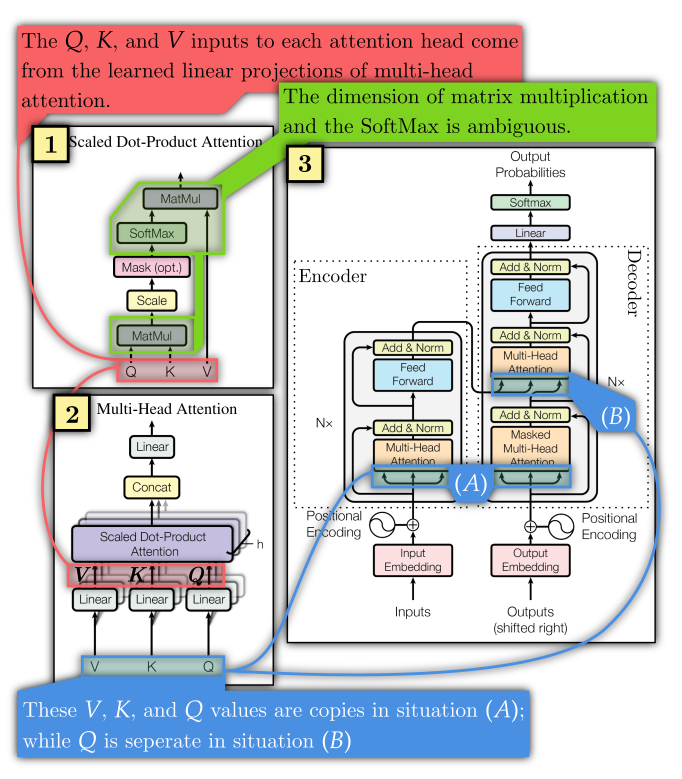
\includegraphics[width=0.6\textwidth,angle=90]{figures/transformer_original.png}
            \caption*{\cite{abbott2024neural}}
        \end{center}
    \end{figure}
\end{frame}

\begin{frame}{Neural circuit diagrams}
    I diagrammi di \textit{deep learning models} generalmente utilizzati nella letteratura scientifica sono inadeguati in quanto non riportano molti dettagli importanti ai fini dell'implementazione (\cite{abbott2024neural,khatri2024anatomy}).
\end{frame}

\begin{frame}{Neural circuit diagrams}
    I \textit{monoidal string diagrams} usati in teoria delle categorie applicata sono inadeguati poiché non riescono a rappresentare funtori e trasformazioni naturali (\cite{abbott2024functor}).
\end{frame}

\begin{frame}{Neural circuit diagrams}
    I \textit{functor string diagrams} prendono ispirazione dai \textit{monoidal string diagrams} e li adattano per rappresentare funtori e trasformazioni naturali (\cite{abbott2024functor}).
\end{frame}

\begin{frame}{Neural circuit diagrams}
    \begin{block}{PRINCIPIO di decomposizione verticale}
        Uno \textit{string diagram} può essere diviso in colonne verticali. Una singola colonna deve contenere solo oggetti o solo morfismi. Colonne con oggetti e colonne con morfismi devono alternarsi.
      \end{block}
      
      \begin{block}{PRINCIPIO dell'espressione equivalente}
        Deve essere possibile sostituire ogni diagramma che segue una nuova notazione grafica con uno diagramma equivalente che segue la vecchia notazione.
      \end{block}

      Vedasi \cite{abbott2024functor}.
\end{frame}

\begin{frame}{Neural circuit diagrams}
    \begin{figure}
        \begin{center}
            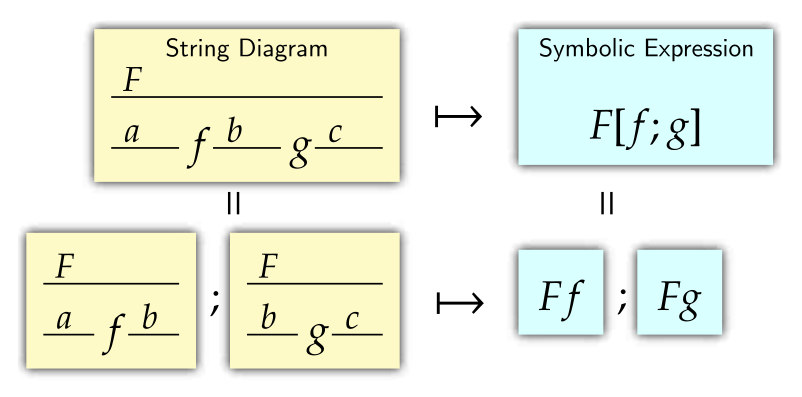
\includegraphics[width=0.9\textwidth]{figures/functors.png}
            \caption*{\cite{abbott2024functor}}
        \end{center}
    \end{figure}
\end{frame}

\begin{frame}{Neural circuit diagrams}
    \begin{figure}
        \begin{center}
            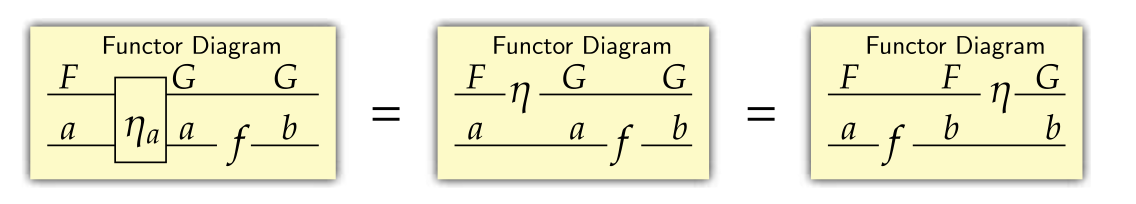
\includegraphics[width=\textwidth]{figures/natural_transformations.png}
            \caption*{\cite{abbott2024functor}}
        \end{center}
    \end{figure}
\end{frame}


\begin{frame}{Neural circuit diagrams}
    \begin{figure}
        \begin{center}
            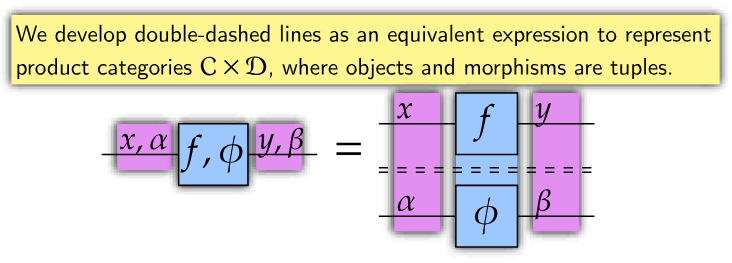
\includegraphics[width=\textwidth]{figures/product_diagram.png}
            \caption*{\cite{abbott2024functor}}
        \end{center}
    \end{figure}
\end{frame}


\begin{frame}{Neural circuit diagrams}
    \begin{figure}
        \begin{center}
            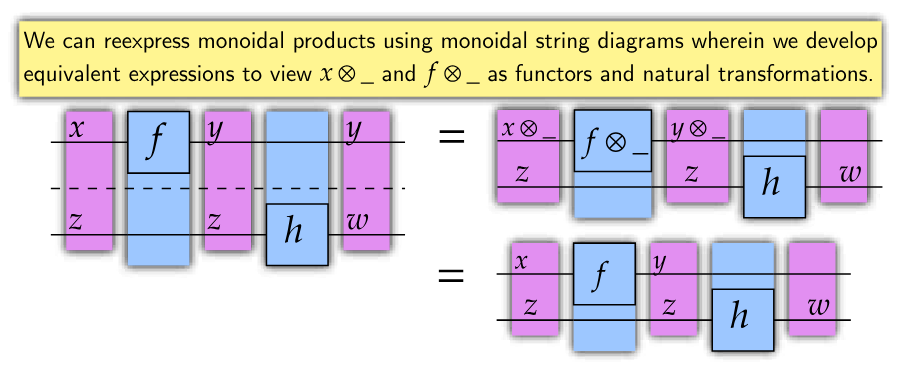
\includegraphics[width=\textwidth]{figures/monoidal_product_diagram.png}
            \caption*{\cite{abbott2024functor}}
        \end{center}
    \end{figure}
\end{frame}

\begin{frame}{Neural circuit diagrams}
    I \textit{neural circuit diagrams} sono \textit{functor string diagrams} specializzati nel rappresentare architetture di reti neurali (\cite{abbott2024functor}).
\end{frame}

\begin{frame}{Neural circuit diagrams}
    \begin{figure}
        \begin{center}
            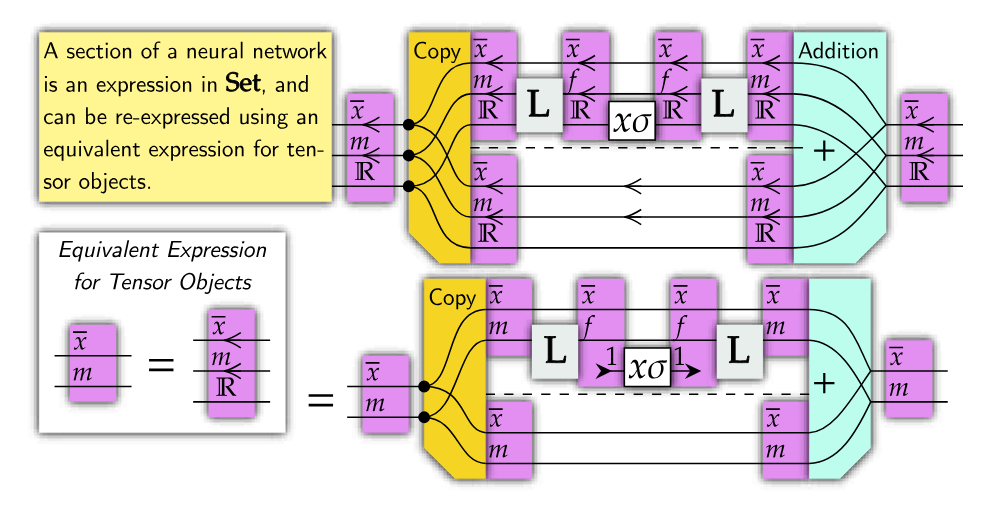
\includegraphics[width=\textwidth]{figures/from_fsd_to_ncd.png}
            \caption*{\cite{abbott2024functor}}
        \end{center}
    \end{figure}
\end{frame}

\begin{frame}{Neural circuit diagrams}
    \begin{figure}
        \begin{center}
            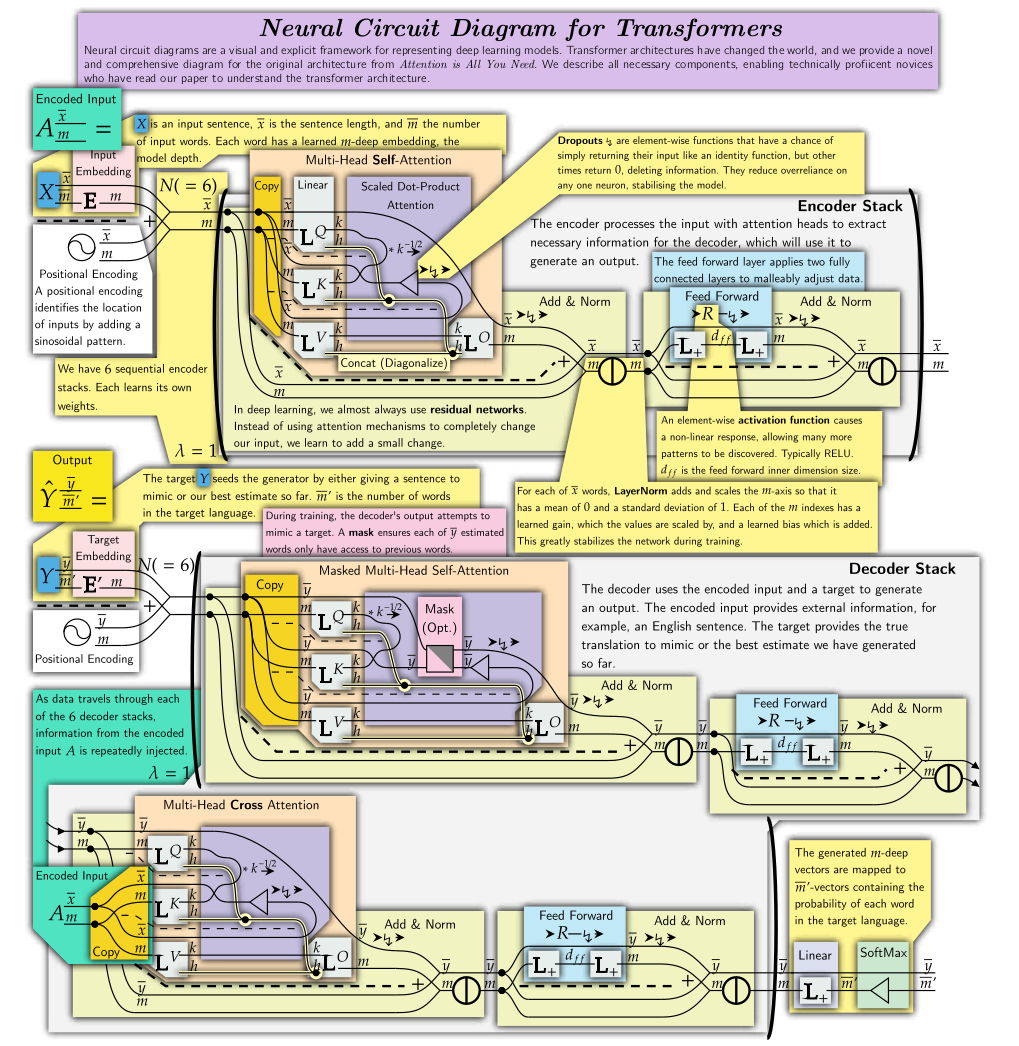
\includegraphics[width=\textwidth]{figures/transformer_ncd.png}
            \caption*{\cite{abbott2023robust}}
        \end{center}
    \end{figure}
\end{frame}

\begin{frame}[standout]
    \huge Prospettive future
\end{frame}

\begin{frame}{Prospettive future}
    C'è una competizione in corso tra varie discipline, che puntano a spiegare le reti neurali utilizzando ciascuna i propri strumenti:
    \begin{itemize}
        \item<1-> \textbf{fisica matematica} {\footnotesize (e.g. \cite{roberts2022principles})},
        \item<2-> \textbf{topologia} {\footnotesize (e.g. \cite{hensel2021survey})},
        \item<3-> \textbf{probabilità} {\footnotesize (e.g. \cite{patel2015probabilistic})},
        \item<4-> e così via...
    \end{itemize}
    
\end{frame}

\begin{frame}{Prospettive future}
    La teoria delle categorie, oltre a offrire strumenti propri, potrebbe creare un ponte tra queste discipline e potrebbe unificare i loro approcci in una teoria generale del deep learning.
\end{frame}

\begin{frame}[allowframebreaks]
    \printbibliography
\end{frame}

\end{document}